\chapter{Results and analysis}
\label{ch:results}

From a qualitative evaluation of the three architectures: Adversarial Anomaly Detector, sVAE, and GM-VAE; the one presenting the best reconstruction is the Adversarial Anomaly Detector. For the two autoencoders, the reconstructions suffer from blurring (see figures \ref{fig:svae_rec} and \ref{fig:gmvae_rec}), making it difficult to evaluate the presence of an anomaly and hence confirming one of the main problems of this kind of autoencoders. The problems in the autoencoders could the caused for the bias the learned data distribution has, due to the simpler data distributions underlying the model.

\begin{figure}[H]
\begin{minipage}{\linewidth}
  \centering
  \begin{tabular}{ccc}
  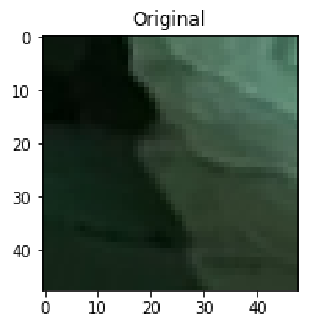
\includegraphics[width=.25\linewidth]{anogan_sample1_original}
    & 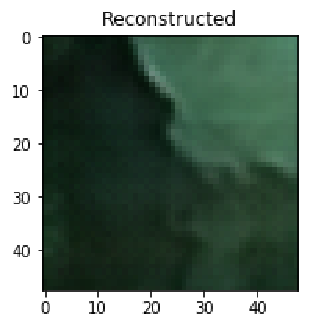
\includegraphics[width=.25\linewidth]{anogan_sample1_reconstruction} \\
  (a) & (b) \\
  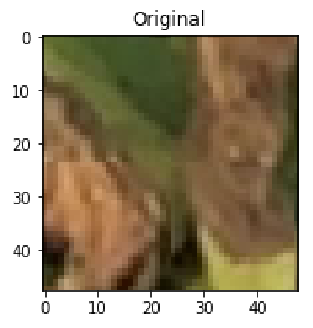
\includegraphics[width=.25\linewidth]{anogan_sample2_original}
    & 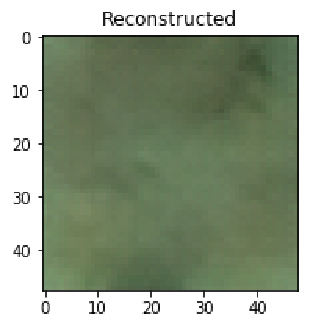
\includegraphics[width=.25\linewidth]{anogan_sample2_reconstruction} \\
  (c) & (d)
  \end{tabular}
  \end{minipage}
\caption[Reconstruction example of the adversarial anomaly detector]{Reconstruction example of the adversarial anomaly detector: a) origianl healthy sample, b) reconstructed healthy sample, c) original test sample and d) reconstructed test sample.}
\label{fig:anogan_rec}
\end{figure}

\begin{figure}[H]
\begin{minipage}{\linewidth}
  \centering
  \begin{tabular}{ccc}
  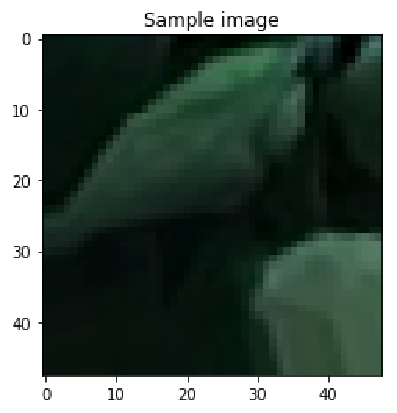
\includegraphics[width=.25\linewidth]{svae_sample1_original}
    & 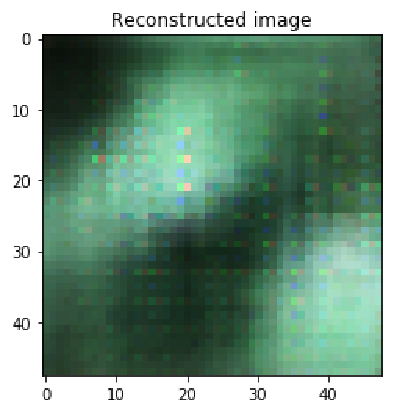
\includegraphics[width=.25\linewidth]{svae_sample1_reconstruction} \\
  (a) & (b) \\
  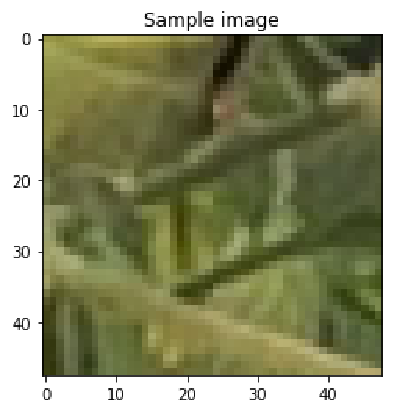
\includegraphics[width=.25\linewidth]{svae_sample2_original}
    & 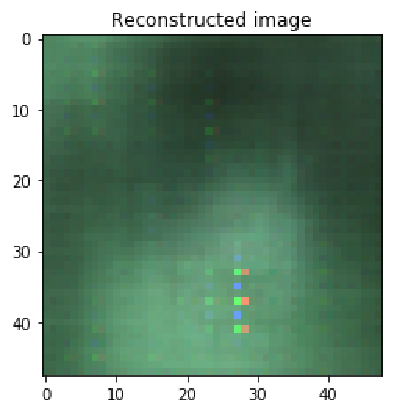
\includegraphics[width=.25\linewidth]{svae_sample2_reconstruction} \\
  (c) & (d)
  \end{tabular}
  \end{minipage}
\caption[Reconstruction example of the sVAE]{Reconstruction example of the sVAE: a) original healthy sample, b) reconstructed healthy sample, c) original test sample and d) reconstructed test sample.}
\label{fig:svae_rec}
\end{figure}

\begin{figure}[H]
\begin{minipage}{\linewidth}
  \centering
  \begin{tabular}{ccc}
  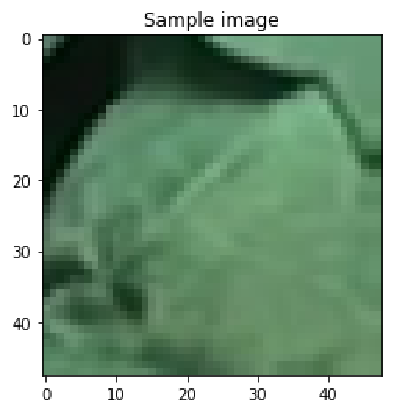
\includegraphics[width=.25\linewidth]{gmvae_sample1_original}
    & 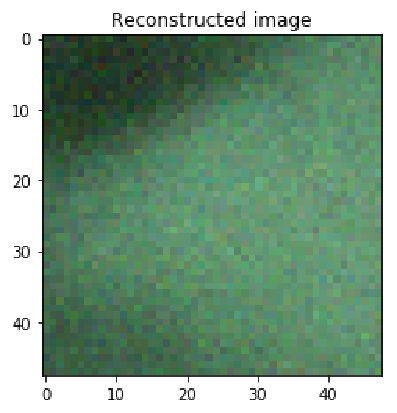
\includegraphics[width=.25\linewidth]{gmvae_sample1_reconstruction} \\
  (a) & (b) \\
  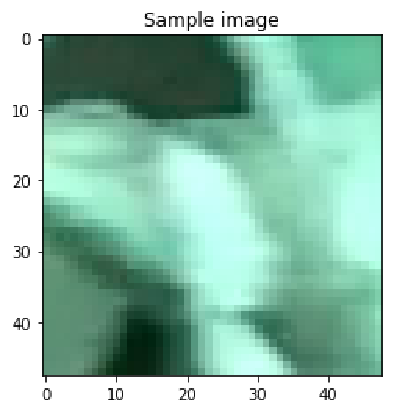
\includegraphics[width=.26\linewidth]{gmvae_sample2_original}
    & 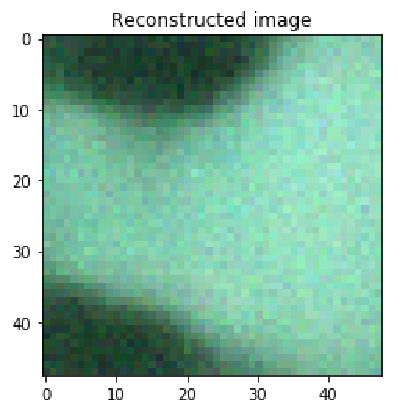
\includegraphics[width=.25\linewidth]{gmvae_sample2_reconstruction} \\
  (c) & (d)
  \end{tabular}
  \end{minipage}
\caption[Reconstruction example of the GM-VAE]{Reconstruction example of the GM-VAE: a) original healthy sample, b) reconstructed healthy sample, c) original test sample and d) reconstructed test sample.}
\label{fig:gmvae_rec}
\end{figure}

\begin{figure}[htb]
  \centering
  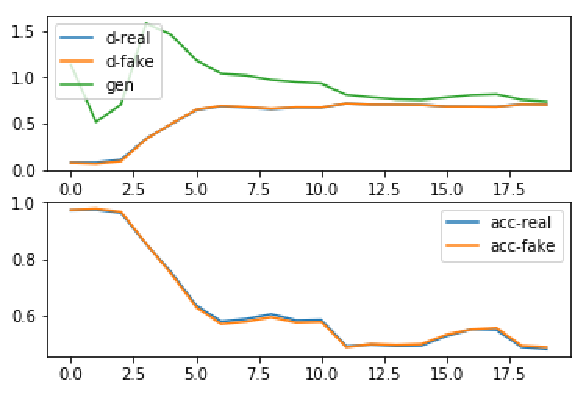
\includegraphics[width=100mm]{gan_training}
  \caption[GAN training]{GAN training: the top graph shows the loss of the generator and the discriminator. The bottom graph shows the accuracy of the discriminator for real and fake images. }
  \label{fig:gan_training}
\end{figure}

The group of healthy samples are extracted from figure \ref{fig:test_images}.a and for the anomalies samples are extracted from figure \ref{fig:test_images}.b. In the case of the AnoGAN, the training of the model is unstable, but with the available tomato data, it was possible to achieve the Nash equilibrium (see figure \ref{fig:gan_training}). The generated images are better than the ones in the autoencoders as can be seen in table \ref{table:rec_eval} with the values of mean and standard deviation (STD) of the healthy and anomaly samples. Its main disadvantage is the time needed to learn a set of latent variables to reconstruct some images. This problem is resolve with the introduction of an encoder in the AnoGAN architecture as shown in the table \ref{table:rec_time} where the reconstruction times are shown for the different models.

\begin{table}[htb]
    \caption[Reconstruction time evaluation]{Reconstruction time evaluation.}
    \label{table:rec_time}
    \centering
    \begin{tabular}{ c c c }
        \hline
        Model & Reconstruction time (ms) \\
        \hline
        sVAE & 160.8 \\
        GM-VAE & 1383.1 \\
        AnoGAN & 6320.6 \\
        Adversarial Anomaly Detector & 255.3 \\
        \hline
    \end{tabular}
\end{table}

Figure \ref{fig:rec_eval} has the reconstruction scores distribution of regular and anomalous samples for the three models. This figure also shows that the best model for the reconstruction of regular samples is the Adversarial Anomaly detector, however, there are still some samples that are indiscernible between regular or anomalous. For that reason explore more metrics would be needed.

\begin{table}[htb]
    \caption[Reconstruction metric evaluation]{Reconstruction metric evaluation.}
    \label{table:rec_eval}
    \centering
    \begin{tabular}{ c c c c c }
        \hline
        Model & Mean (healthy) & STD (healthy) & Mean (anomalies) & STD (anomalies) \\
        \hline
        sVAE & 10410.6 & 7020.3 & 19858.8 & 18464.1 \\
        GM-VAE & 15162.2 & 7597.3 & 9357.3 & 6071.7 \\
        AAD & 3839.5 & 3251.1 & 8996.1 & 3308.8 \\
        \hline
    \end{tabular}
\end{table}

\begin{figure}[H]
\begin{minipage}{\linewidth}
  \centering
  \begin{tabular}{ccc}
  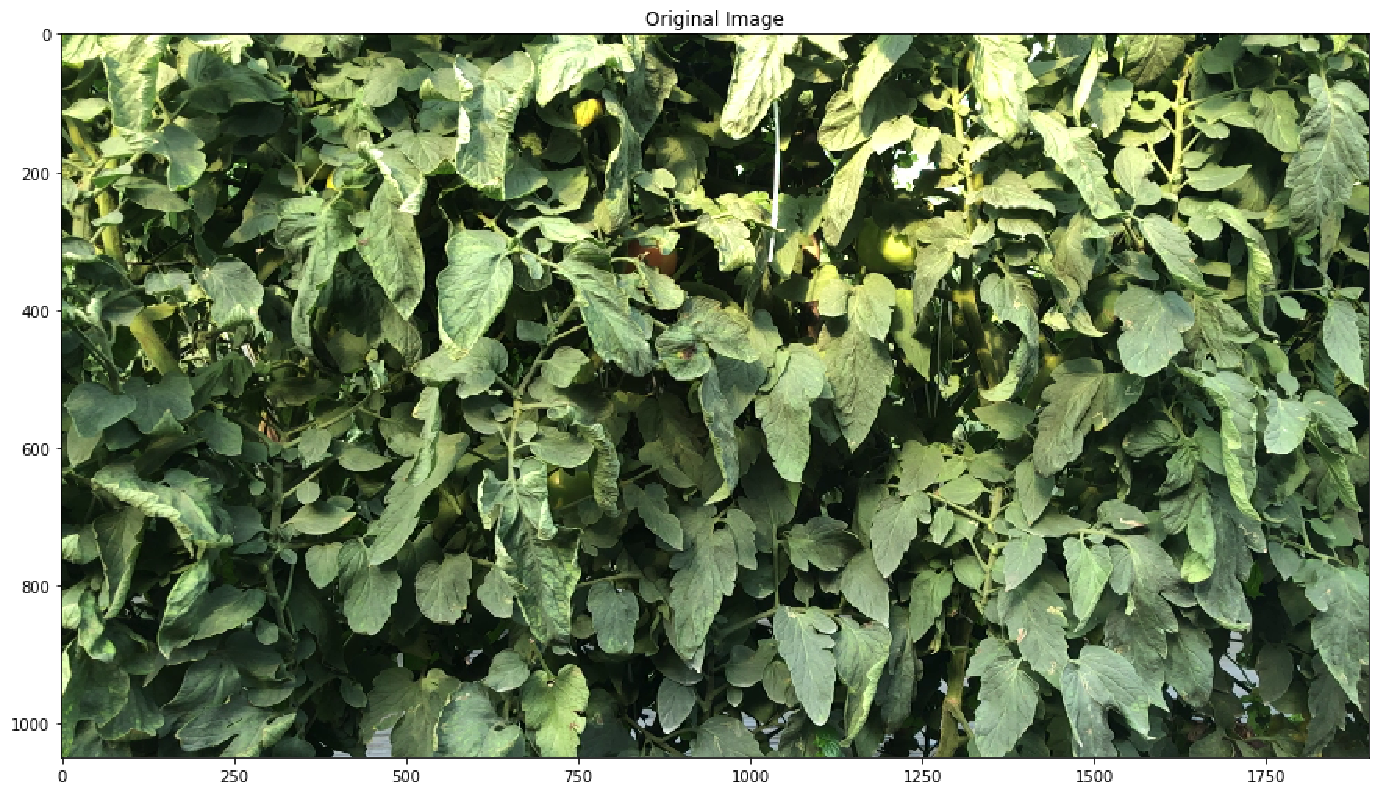
\includegraphics[width=125mm]{anogan_test_image1} \\
  (a) \\ 
  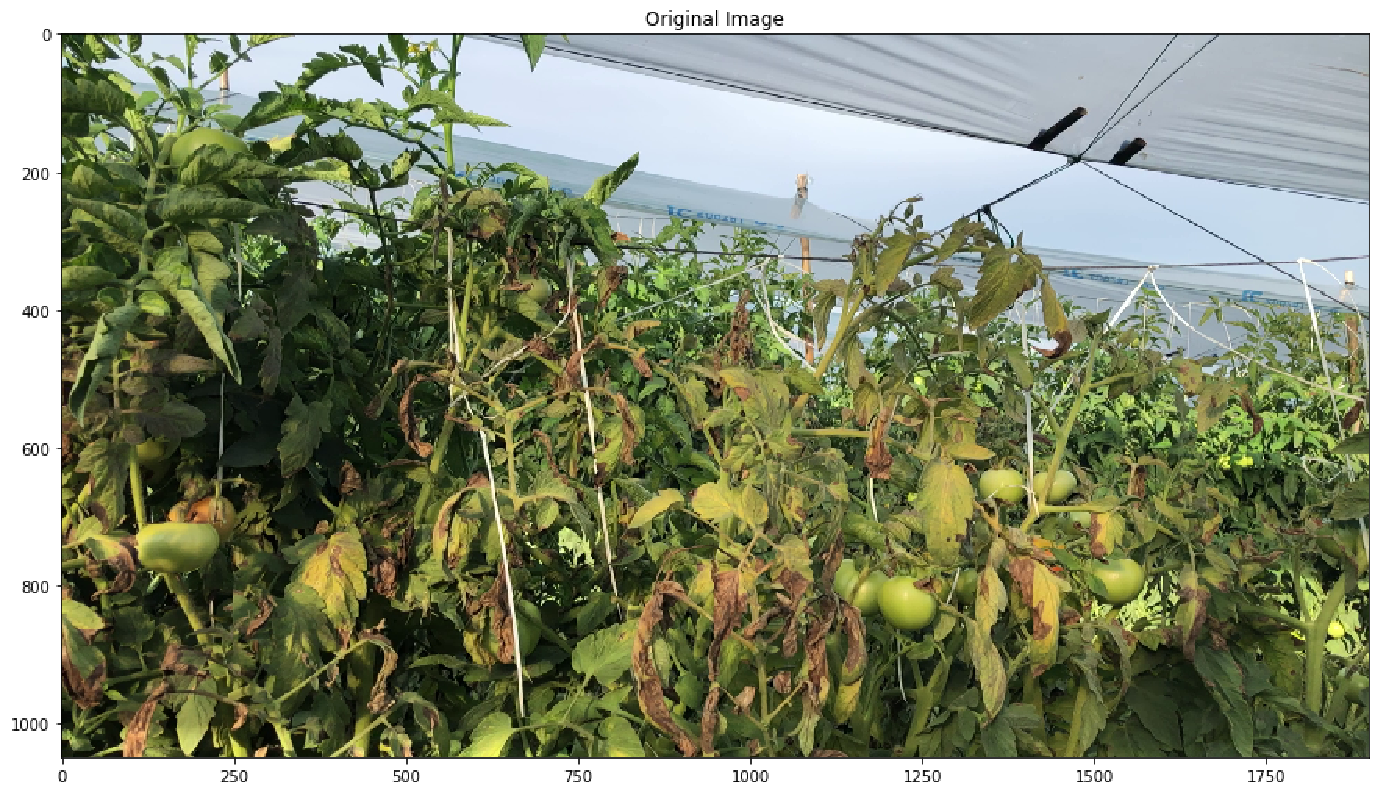
\includegraphics[width=125mm]{anogan_test_image2} \\
  (b) \\
  \end{tabular}
  \end{minipage}
\caption[Experiment test images]{Experiment test images: a) healthy image and b) anomlous image.}
\label{fig:test_images}
\end{figure}

In figures \ref{fig:anogan_eval_test_image_1} and \ref{fig:anogan_eval_test_image_2} depict the data distribution between regualr and anomalous samples. Figure \ref{fig:anogan_eval_test_image_1} shows a defined group of data that represents the healthy samples and a smaller amount of points around this healthy group that represents anomalous data. In figure \ref{fig:anogan_eval_test_image_2} we have the opposite case, where the number of anomalies is larger than the number of healthy samples. For the first case, the test images depict a tomato plant in a healthy state, and for the second case, the tomato plant presented several affections, fact that is reflected in each of the graphs mentioned before.

\begin{figure}[h]
\begin{minipage}{\linewidth}
  \centering
  \begin{tabular}{ccc}
  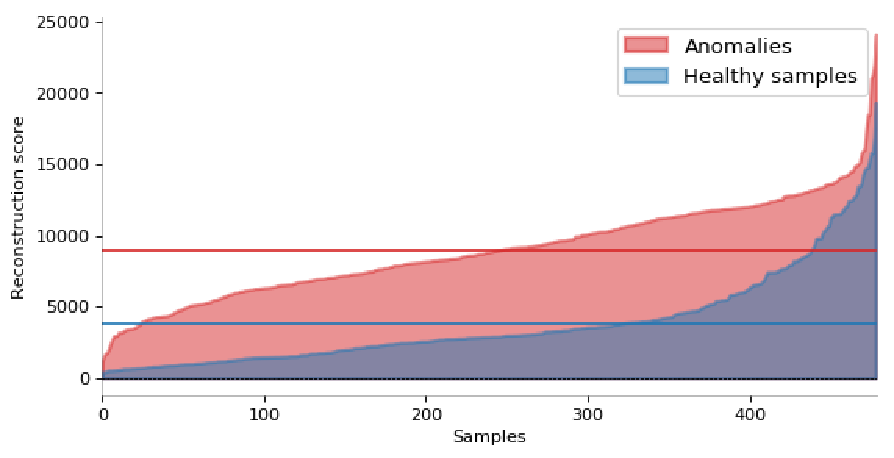
\includegraphics[width=120mm]{rec_anogan_eval} \\
  (a) \\ 
  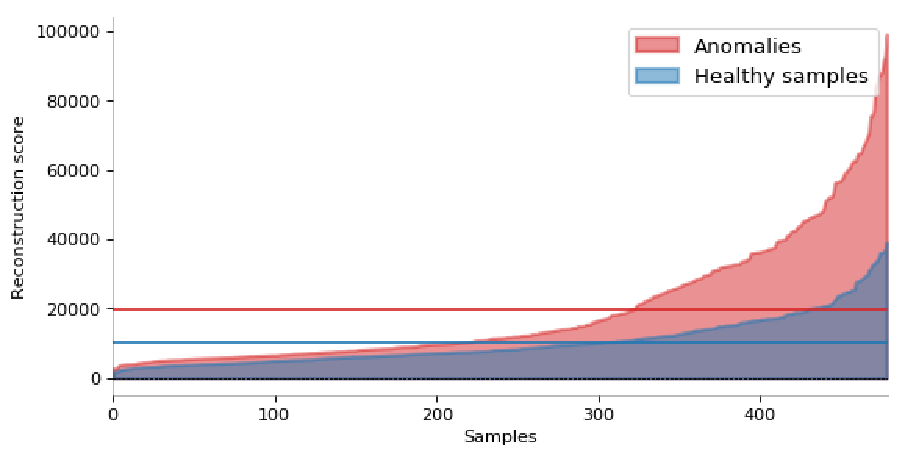
\includegraphics[width=120mm]{rec_svae_eval} \\
  (b) \\ 
  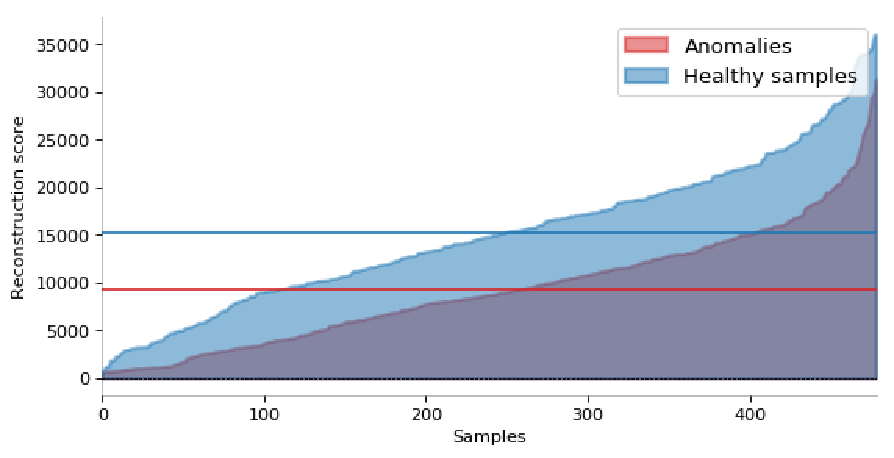
\includegraphics[width=120mm]{rec_gmvae_eval}\\
  (c) \\
  \end{tabular}
  \end{minipage}
\caption[Reconstruction evaluation of the Adversarial Anomaly Detectof, sVAE and GM-VAE]{Reconstruction evaluation of the a) Adversarial Anomaly Detectof, b) sVAE and c) GM-VAE. The horizontal lines represents the mean value of the healty samples and the anomaly samples.}
\label{fig:rec_eval}
\end{figure}

\begin{figure}[htb]
  \centering
  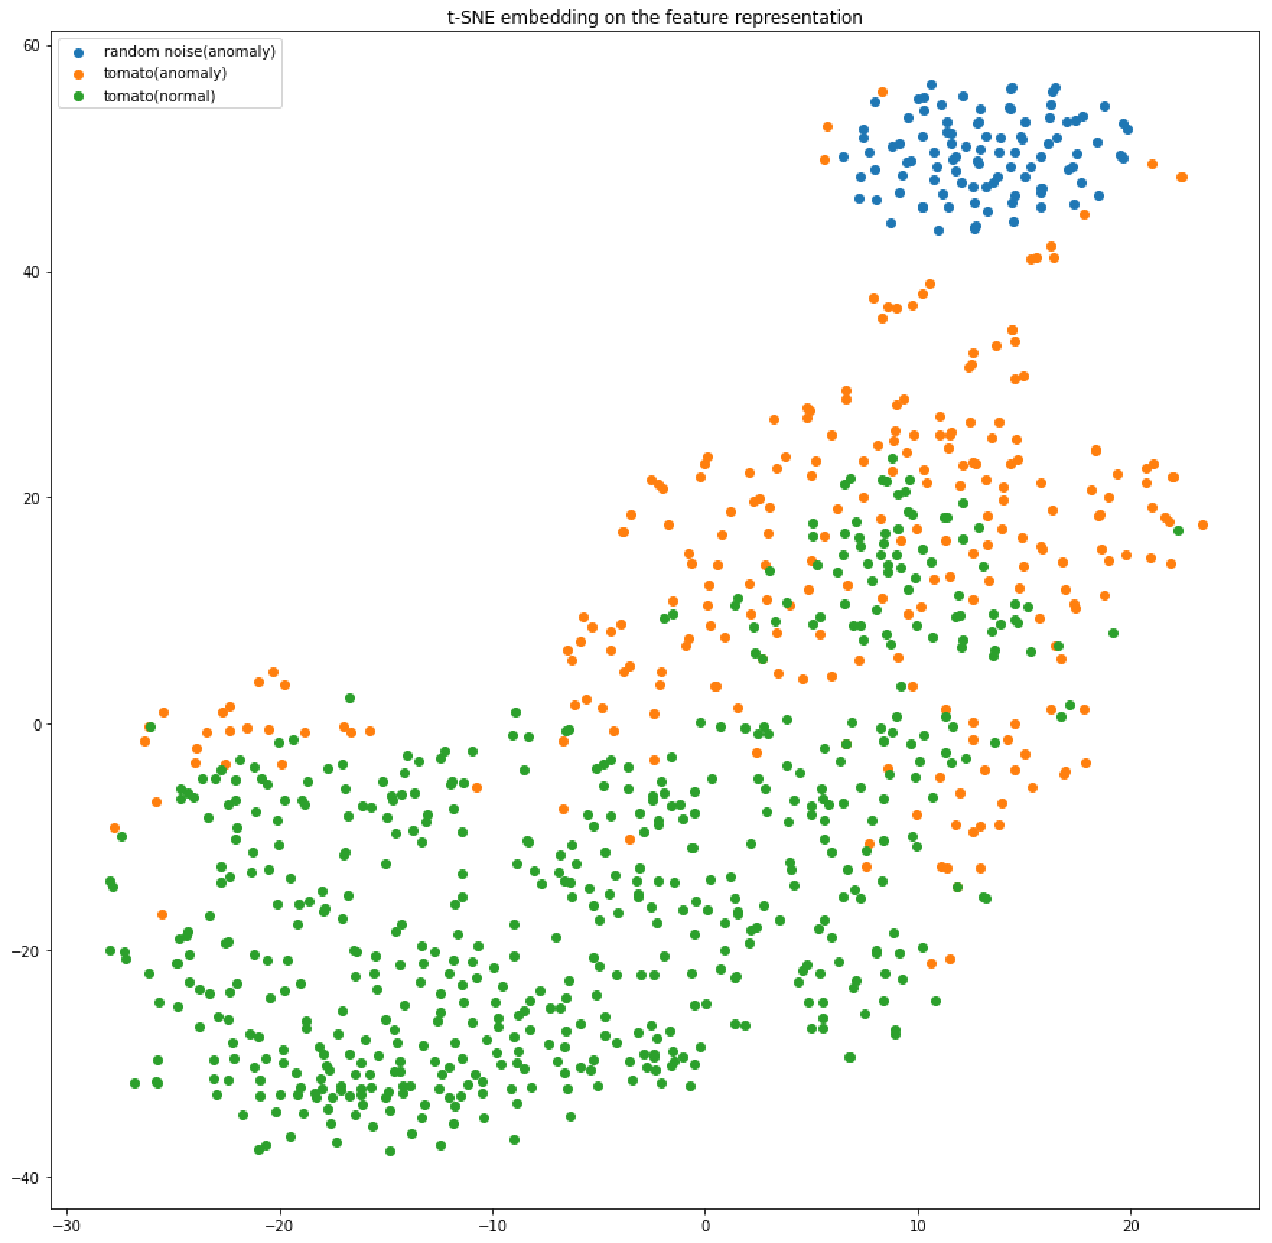
\includegraphics[width=150mm]{anogan_t_sne1}
  \caption[Adversarial Anomaly Detector t-SNE evaluation of test image 1]{Adversarial Anomaly Detector t-SNE evaluation of test image 1}
  \label{fig:anogan_eval_test_image_1}
\end{figure}

\begin{figure}[htb]
  \centering
  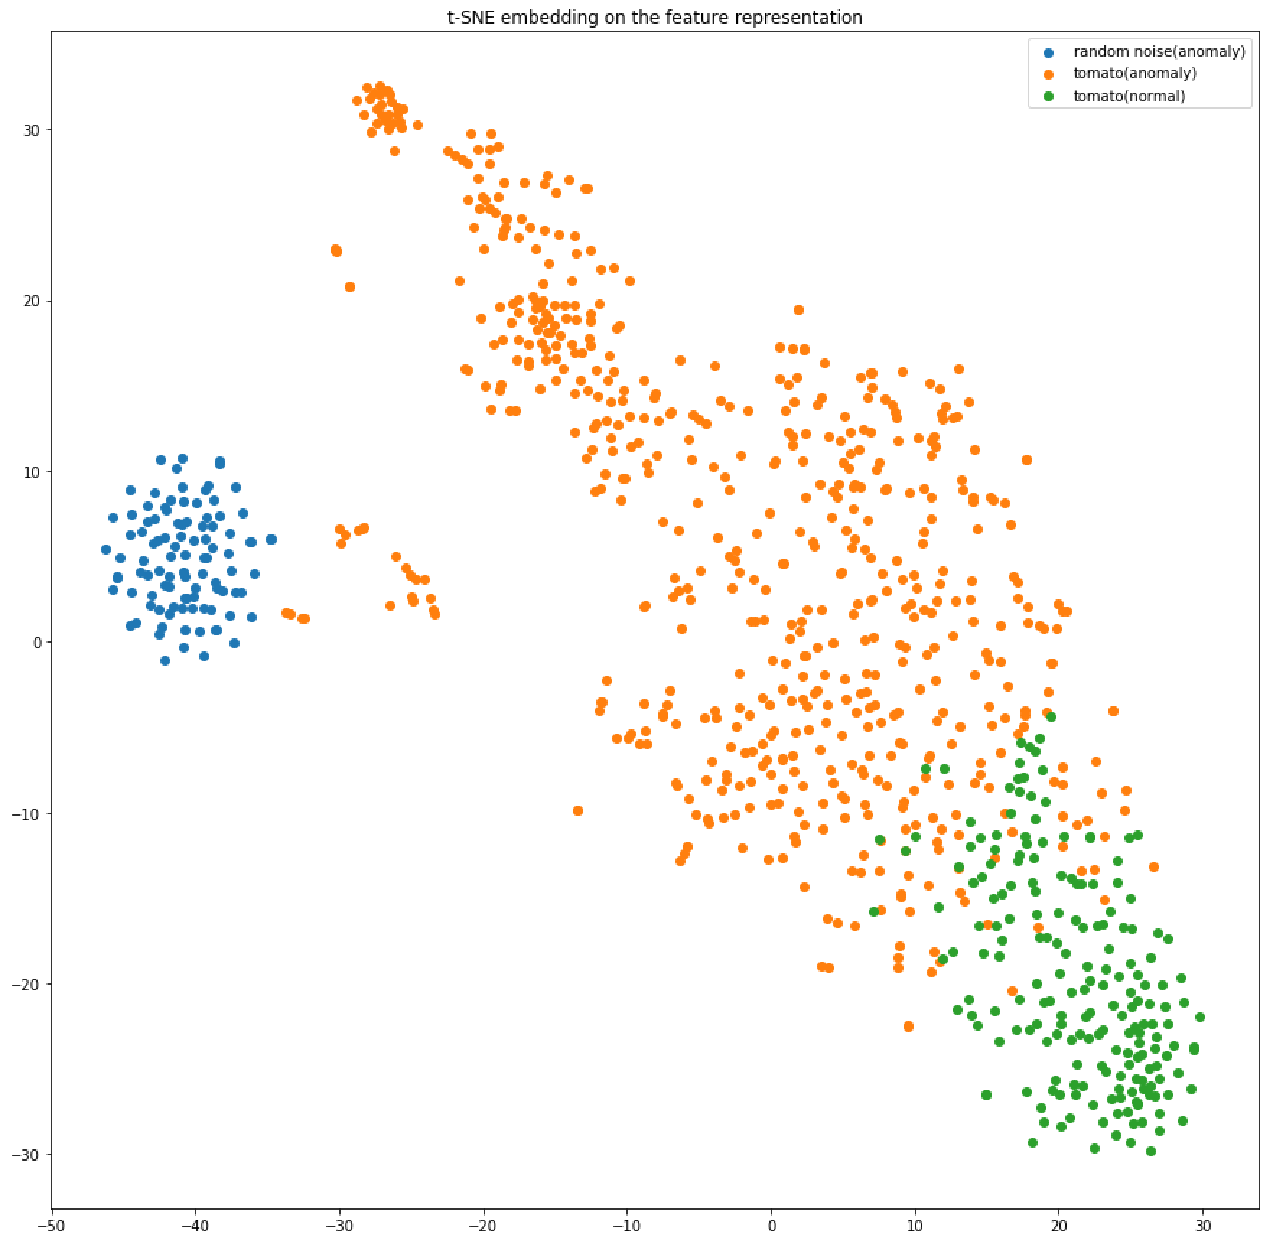
\includegraphics[width=150mm]{anogan_t_sne2}
  \caption[Adversarial Anomaly Detector t-SNE evaluation of test image 2]{Adversarial Anomaly Detector t-SNE evaluation of test image 2}
  \label{fig:anogan_eval_test_image_2}
\end{figure}
